\subsection{Shared state: \textit{libgotcha}}
\label{sec:libgotcha}

Although shared state is always a problem for preemptible functions, we classify code
that relies on shared state depending on its location:\@ we term it \textbf{internal
stateful code} if it is part of a project (i.e., in the same linked object file)
that uses preemptible functions, and \textbf{external stateful code} otherwise (e.g.,
as is the case for third-party libraries).  Recall that one of our goals is to
support third-party libraries without needing to recompile them.

We begin by briefly discussing internal stateful code.  Figure~\ref{fig:ingerbug} shows
a code passage with a concurrency bug:\@ because the \texttt{timed()} function does
not use an atomic increment operation, its \texttt{launch()} invocation might be
preempted after reading the \texttt{count} variable but before writing it, in which
case the \texttt{resume()} will set the value back to \texttt{1}, causing
the assertion to fail.  We take the stance that internal stateful code is responsible
for implementing its own concurrency control to fix this kind of problem, since the
developers are aware they are using preemptible functions, and therefore (hopefully)
are also aware of the concurrency implications.  If the internal stateful code were
written in Rust instead of C, the compiler would statically prevent many such bugs by
forcing the user to use atomics or locks to protect shared variables such as
\texttt{count}.

\begin{figure}
\begin{verbatim}
static int count = 0;

static void *timed(void *ignored) {
  ++count;
  return NULL;
}

int main(void) {
  struct linger res =
    launch(timed, VERY_SHORT, NULL);
  ++count;
  resume(&res, LONG_ENOUGH);
  assert(count == 2); // BUG!

  return 0;
}
\end{verbatim}
\caption{Concurrency bug in internal stateful code}
\label{fig:ingerbug}
\end{figure}

The problem we do have to handle is external stateful code, since there's no way an
existing piece of code can be expected to know that it might be called from a
preemptible function.  In other words, the developers of libraries such as
\texttt{libc} should not need to know that preemptible functions exist.  On the other
hand, we cannot restrict programs that use preemptible functions to calling only
async-signal-safe functions.  This is where libgotcha comes in:\@ it detects possible
external stateful code at runtime by instrumenting the
boundaries between relocated ELF object files (i.e., executables and dynamic shared
objects).

To avoid both limitations, we slightly weaken the guarantees of either dynamic
linking or preemption, depending on the scenario.  In the common case, we weaken the
property that every use of a dynamically-linked function or global variable resolves
to the same address:\@ we open multiple copies of the shared objects required by the
application, and redirect uses of libraries' symbols to a separate copy for each
preemptible function.  In this way, we ensure that inconsistent state from a library
used by one preemptible function cannot affect uses of that same library by other
preemptible functions or the broader application.  Although this approach works for
many
libraries, it is sometimes inappropriate; for instance, using multiple copies of the
dynamic allocator would cause them to manage the same heap with different free lists.
In such cases, we direct all dynamic calls to the same copy of the function and defer
preemption on that kernel thread until the call has completed, in the style of
goroutines.

We refer to each independently-loaded copy of all the program's object files as a
\textbf{libset}.  The libgotcha library exposes a per-thread attribute called the
\textbf{current libset} that controls the libset serving all uses of library code.
(Note that this does not determine the libset from which the current code is being
executed.)   This attribute is set to the main libset whenever the flow of control is
outside any preemptible function; otherwise, it is set to a value specific to that
function.  Thus, each preemptible function's library calls are isolated from those in
the rest of the application.  In the event that a preemptible function must be
canceled while it is executing within its libset, the latter can be reinitialized by
closing all its loaded objects, then reopening them to prepare it for reuse.  Note
that, in principle, libgotcha functions with an unmodified GNU dynamic linker.

\paragraph{Dynamic linking}

A key feature of shared libraries is the ability to replace them between the time an
application is built and when it is executed.  This is enabled by dynamic linking, an
approach by which the static linker delays the relocation of addresses associated
with \textbf{dynamic calls} to functions and \textbf{dynamic references} to global
variables.  Instead of resolving their addresses directly within the output machine
code, the static linker includes a
\textbf{dynamic relocation table} in each output ELF object file describing the
locations of dynamic calls and references, as well as the name of each target symbol.
A component of the C runtime known as the dynamic linker (\texttt{ld.so}) uses this
table to resolve dynamic symbol addresses after the application is loaded.

It is important to realize that dynamic calls and references are resolved based on
the name of a symbol, which may be ambiguous between multiple libraries; as such, the
library associated with each dynamic relocation is not determined until runtime.
In fact, a dynamic relocation might even resolve back to the same object file that
contains it; this is most common when a shared library makes an internal reference to
one of its own public interfaces (since the application might replace that public
interface with its own implementation or one from a different library).  The target
of dynamic relocations will become important for our discussion, so we term them as
\textbf{cross-library references} or \textbf{cross-library calls} if the target
symbol ends up being located in a different object file than the use.

\paragraph{GOTs and PLTs}

When a dynamically-linked executable is run, the kernel first passes control to the
dynamic linker, which loads all required shared object files and populates their
respective \textbf{global offset tables (GOTs)}\footnote{It is from these structures
that \textit{lib\textbf{got}cha} gets its name.} with the resolved addresses of any
referenced dynamic symbols.  Once program loading is complete, the GOT entries
for any dynamic references to global variables are populated with those variables'
true addresses.

Dynamic calls to functions are slightly more complicated because they can resolve
lazily at first invocation.  For instance, the instruction
\texttt{call~printf@plt} causes the assembler to generate a corresponding executable
\textbf{procedure linkage table (PLT)} stub function, as shown in
Figure~\ref{fig:plt}.  The first instruction of this stub looks up the address of the
function by checking a corresponding GOT entry; however, initially this contains the
address of the immediately-following \texttt{pushq} instruction!  Thus, on the first
call, the PLT stub pushes a symbol relocation identifier (here, \texttt{0x0}) onto
the stack and calls into the dynamic linker, which resolves the symbol to the
function's real address, memoizes the result by updating the GOT entry, and finally
jumps into the real function.  Subsequent calls to the PLT stub then forward to the
real function after executing only the initial \texttt{jmpq} instruction.

\begin{figure}
\begin{verbatim}
0000000000001030 <printf@plt>:
  1030:  jmpq   *0x2fe2(%rip) <printf>
  1036:  pushq  $0x0
  103b:  jmpq   1020 <.plt>
\end{verbatim}
\caption{Example PLT entry for call to \texttt{printf()}}
\label{fig:plt}
\end{figure}

\paragraph{Intercepting cross-library calls}

\solb{Mention the need to \texttt{mprotect()}?}

The primary objective of the libgotcha library is to maintain multiple copies of each
loaded ELF object file and seamlessly direct each use at the correct one.  It does
this by altering GOT entries to trick the PLT stubs into injecting libgotcha code at
the beginning of each cross-library call.  The GNU
dynamic linker includes a feature known as namespaces~\cite{dlmopen-manpage},
inherited from Solaris, that allows loading multiple copies of the same object file
at runtime; however, it treats each namespace as a completely independent dependency
graph of loaded objects, with no relationship to any other.  We built
libgotcha on top of namespaces, to which it adds automatic routing of function calls
and variable references between separate namespaces; it is these augmented
namespaces that we refer to as libsets.  Specifically, libgotcha creates a fixed
number of
libsets, each of which can be reused as long as no calls into it from the same thread
of execution are allowed to interleave.

In order to use the libgotcha library, a program need only link against its shared
library, which contains a constructor that the dynamic linker will invoke as soon as
it has finished loading all the program's library dependencies.  The constructor
should not instrument all dynamic calls because this would
have inconsistent semantics in the case of object files with self-referential dynamic
relocations, since there is no easy way to instrument static calls at runtime.
(Consider how confusing it would be if a shared library making calls to its own
static helper function and its own public function had those calls implicitly
redirected to different
copies of itself.)  Instead, we make the decision to only switch libsets on
cross-library dynamic calls.

Before updating any GOT entries, we must identify
which ones correspond to cross-library calls.  Doing this is a multi-step process:
First, we traverse the relocation table for each loaded object file, cross
referencing each of its relocation entries against the local object file's symbol
table.  If the symbol table does not contain a definition matching the relocation
entry's target, we conclude that the relocation must correspond to a cross-library
call.  Otherwise, we check the address in the GOT entry corresponding to the
relocation entry:  If this address is outside the bounds of the current object file,
it is a cross-library call.  Otherwise, if this address matches the one from the
symbol table entry, it is not a cross-library call, and should be skipped.  The last
case is the trickiest, since the GOT entry probably still refers to the PLT stub
(because the symbol reference has not yet been resolved).  In this case, we resolve
the symbol
early, update the GOT entry, and recheck whether it resolved to the local definition
to determine whether it is a cross-library call.

Next, the constructor allocates one or more executable pages full of custom PLT-like
stubs, which we refer to as the \textbf{procedure linkage override tables (PLOTs)}.
Each PLOT is associated with one \textbf{shadow GOT} for each namespace:\@ when a
particular PLOT stub is executed, it pushes an index to the stack and calls a
function, \texttt{procedure\_linkage\_override()}, that decides which libset the call
should target, locates the corresponding shadow GOT, and transfers control to the
address listed at the appropriate index in that table.  (Because this function
is injected into the "middle" of function calls, it is written in assembly to avoid
clobbering any of the application's registers.)  The constructor sets up this system
by replacing each GOT entry corresponding to a cross-library call with a fresh PLOT
entry, storing its previous value in the shadow GOT for the main namespace.  It
then opens another copy of each library in each namespace, redirects its
cross-library calls to the same PLOT stubs, and creates a shadow GOT for each
namespace.

The setup procedure described so far has one significant problem:\@ recall that a PLT
call memoizes the real address of its symbol by replacing the GOT entry, which should
cause subsequent calls to skip libgotcha's \texttt{procedure\_linkage\_override()}
codepath.  In order to prevent this, the constructor updates the relocation entries
corresponding to cross-library calls to point at \textit{shadow} GOT entries.  This
fools the dynamic linker into updating the shadow entry instead, meaning that
memoization still works, as shown in Figure~\ref{fig:override}.

\begin{figure}
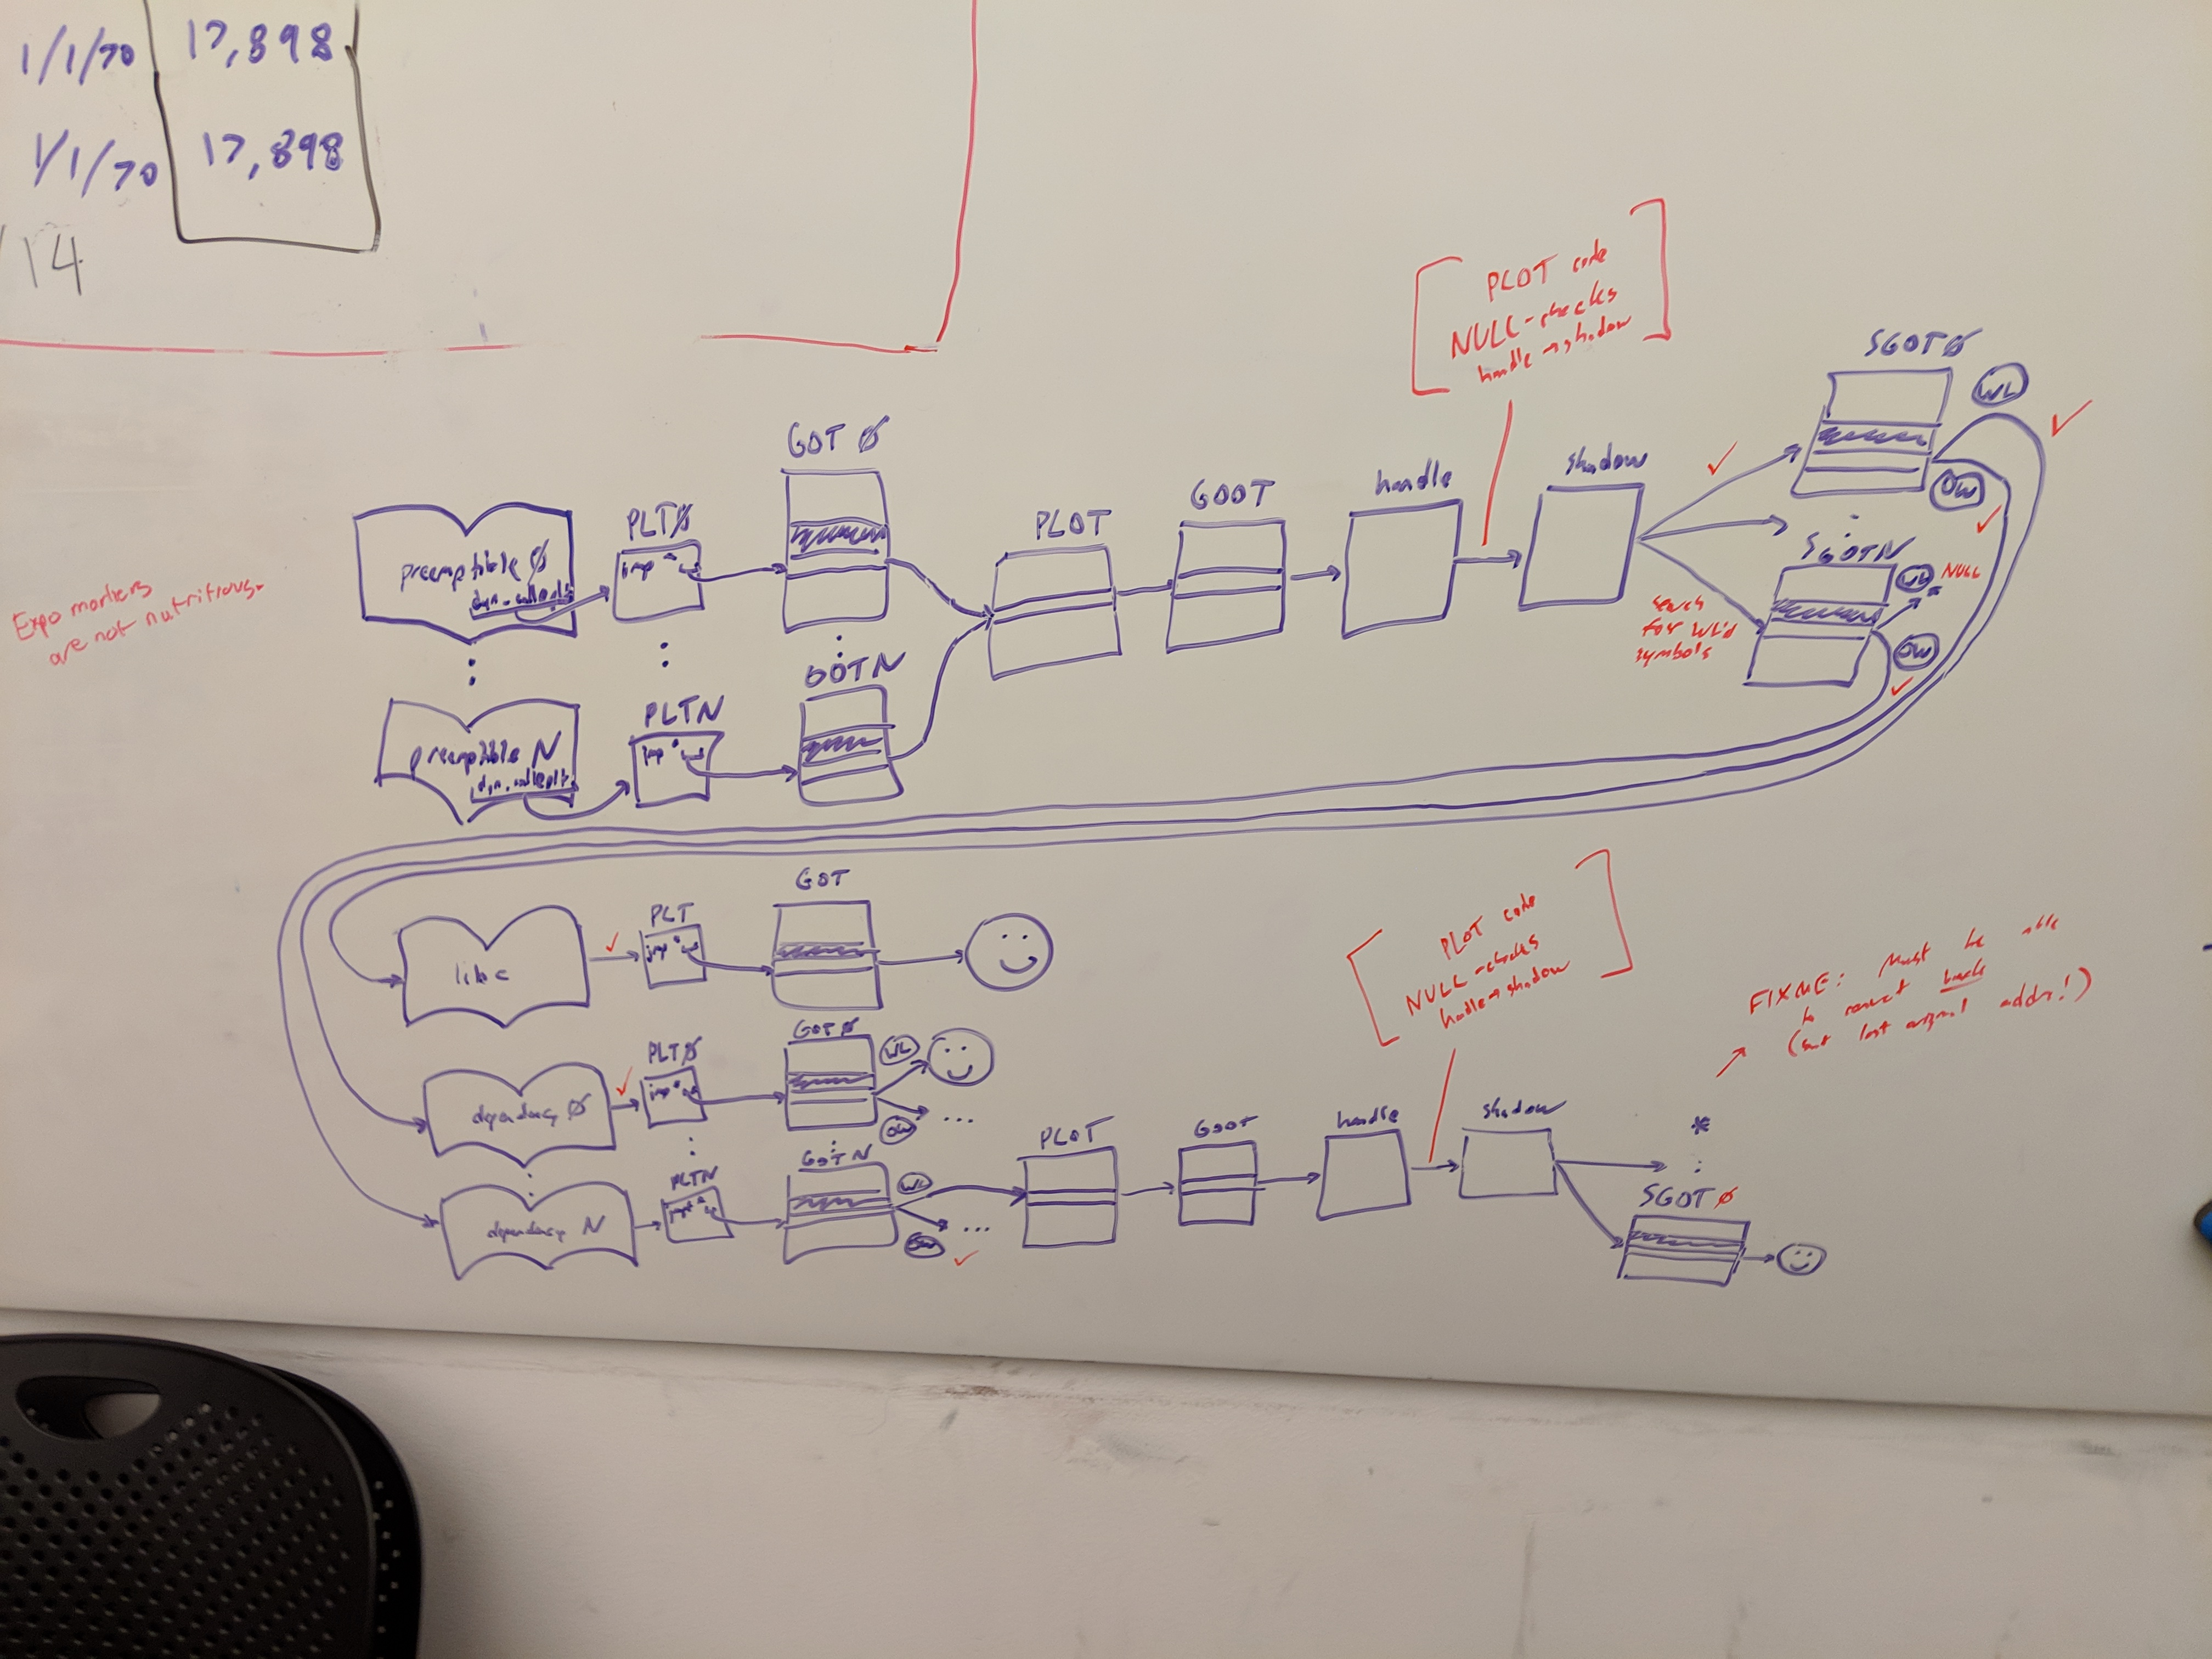
\includegraphics[width=\columnwidth]{figs/tables}
\caption{\texttt{procedure\_linkage\_override()}'s table lookups}
\label{fig:override}
\end{figure}

\paragraph{Incercepting cross-library references}

The reader might notice that invocation is not the only thing a program can do with a
function:\@ it might also pass around the function's address.  In fact, after taking
the address, it could pass it to code within a different object file, which might
compare it.  In order for such comparisons to correctly indicate whether the same
code will be run, the compiler loads such addresses directly from the GOT via
instructions of the special position-independent relocation form
\texttt{mov~\textit{symbol}@gotpcrel(\%rip),~\%\textit{dest}}, and the dynamic linker
resolves the calls and populates their GOT entries eagerly at load time.  To avoid
breaking pointer-comparison semantics, libgotcha makes sure to share the same PLOT
stub between all GOT entries to a given symbol that use this type of
relocation.  As long as the current libset remains the same between the time of a
function pointer comparison and the time of its invocation, such a comparison
guarantees that \texttt{procedure\_linkage\_override()} will dispatch to the same
copy when invoked using either pointer.

Handling references to global data besides functions is more challenging, and less
efficient, because such accesses use the aforementioned position-independent
relocation but don't include a PLT-style codepath for us to co-opt.
In order to capture (hopefully rare) cross-library references to global variables,
we use a different approach.  After each shadow GOT page, we allocate an inaccessible
page with no protection bits set.  Each time the libgotcha constructor encounters a
relocation entry corresponding to a data symbol, we migrate the contents of its GOT
entry into an available shadow GOT entry, replacing it with an address the same
number of bytes into the shadow GOT's corresponding inaccessible page.  Thus,
whenever the program takes the address of a particular symbol, it gets the same fake
address.  Any attempt to read from or write to this address results in a segmentation
fault, which libgotcha catches; we then look up the real address in the shadow GOT
corresponding to the currently-selected libset, disassemble the offending
instruction(s), and replace the contents of the memory-address register with the
found address.  Once the signal handler returns, the instruction executes again, this
time with a valid memory address in its register.  Although it's possible to generate
code sequences that are incompatible with this approach (e.g., because they perform
in-place pointer arithmetic on a register rather than using displacement-mode
addressing with a base address), in our experience public shared data is rare enough
that we haven't yet encountered any cases where programs do this.

\paragraph{Shared symbols}

As aforementioned, certain systems such as the dynamic memory allocator do not work
well when copied, and must be treated specially.  Specifically, libgotcha maintains
a whitelist of \textbf{shared symbols} whose use is always redirected back to the
main namespace.  Of course, this introduces prior work's limitation of being unable
to preempt during such calls; as such, the whitelist should be kept small, since the
inclusion of each function confers trust in its timely completion.

When whitelisting the dynamic allocator, it is important not to whitelist all of libc
as collateral damage,
since preemptible functions could easily exploit this to run forever (e.g., by
performing their work in the \texttt{qsort()} function's comparator callback).
Fortunately, libc uses dynamic calls when it needs to invoke the allocator
internally, allowing us to whitelist that component alone.

In order to support more complex systems, libgotcha exposes a simple API for dealing
with shared symbols.  Whenever \texttt{procedure\_linkage\_override()} transfers
control to the main libset, it resets the current libset so that all subsequent calls
will remain in shared code.  Client code can therefore check the current libset to
determine
whether it is safe to preempt.  Furthermore, libgotcha provides an interface by which
client code can provide a callback to be invoked upon return from the shared code,
immediately after the transition back to the original libset:\@ it can use this
callback to perform a deferred preemption check at the earliest possible point.

The attentive reader will observe that, in order to track the current libset,
libgotcha must itself contain shared state.  In order to ensure a consistent view of
this information independent of the current libset, it treats all the symbols from
its own shared library as shared by automatically appending them to the whitelist.

\paragraph{Shortcomings and workarounds}

The libgotcha approach has known conflicts with two modern extensions to the
dynamic-linking model.  Here we discuss these shortcomings and our proposed
workarounds.

When an executable directly accesses a global variable defined in a shared library,
the assembler migrates it into the executable, allowing the main program to access it
via static relocations instead of via the GOT.  The static linker generates a COPY
relocation that causes the dynamic linker to copy the variable's contents from the
shared library at load time.  Unfortunately, this approach makes
it impossible for us to intercept cross-library references occurring within the
executable, and causes associated dynamic references in the defining shared library
to be erroneously treated as cross-library references.  For this reason, libgotcha
emits a warning when it detects a COPY relocation.  Developers can avoid the problem
by building any executables that use libgotcha with the C compiler's \texttt{-fpic}
flag to skip generating such relocations.

Some shared libraries are marked with a special configuration flag,
\texttt{DF\_1\_NODELETE}, which prevents the dynamic linker from ever removing them
once they've been loaded.  Because almost all libraries depend on libc, the presence
of even one such library prevents us from reinitializing a libset for reuse after
its preemptible function has been canceled!  The flag is mostly used on libraries
that need
to monkey-patch some other loaded library, such that the two subsequently have a
circular dependency.  Fortunately, this is not usually a problem because when we
unload one library from a libset, we then unload the rest, so whenever we encounter a
\texttt{NODELETE} object file, we make a special copy with the flag cleared, for
loading into every namespace except the main one.  The one place this doesn't work is
when a library monkey-patches the dynamic linker itself.  This
requires the use of a private interface, and the only offending library to our
knowledge is GNU libpthread, which replaces function pointers in order to cause the
dynamic linker to take locks when performing potentially concurrent operations; we
handle this by preventing the monkey-patching constructor code from running in our
modified copy of that library.

\subsection{Case study: Auto async-signal safety}
\label{sec:statefulness}

The main use of libgotcha is to make library function calls async-signal safe when
they wouldn't otherwise be.  We now pause to give a brief example of such usage,
motivated by the buggy program in Figure~\ref{sec:handlerbug}, which calls the
async-signal-unsafe function \texttt{printf()} from its signal handler.
Unfortunately, this function takes a lock on the \texttt{stdout} stream's associated
file descriptor, and the signal handler eventually interrupts the program within
\texttt{fflush()} while it is holding this same lock, resulting in deadlock.

\begin{figure}
\begin{verbatim}
static void handler(int ignored) {
  printf("in signal handler()\n");
}

int main(void) {
  struct sigaction sa = {
    .sa_handler = handler,
  };
  sigaction(SIGALRM, &sa, NULL);

  struct timeval tv = {
    .tv_sec = 1,
  };
  struct itimerval it = {
    .it_interval = tv,
    .it_value = tv,
  };
  setitimer(ITIMER_REAL, &it, NULL);

  while(true)
    fflush(stdout);
}
\end{verbatim}
\caption{C program with a buggy signal handler}
\label{sec:handlerbug}
\end{figure}

There are two ways to weaken the semantics of this program to prevent the deadlock
without modifying the program's source code.  (1) We can elide the file descriptor
lock, which in this case may occasionally allow the signal handler's output to
interleave with any (hypothetical) output from the main program (if the signal
handler interrupts a \texttt{write} syscall from the stream library implementation).
(2) We can defer handling of any signal that arrives during a call to
\texttt{fflush()} until that function returns.

In 127 lines of C, we wrote a signal-handling client library, \textit{libas-safe},
that can use libgotcha to automatically transform the program in either of these
ways.  It injects code before \texttt{main()} to switch to a new libset, and
provides a custom implementation of \texttt{sigaction()} that switches the current
libset back to the main one while each signal handler is running.  This is enough to
achieve transformation (1), since it causes \texttt{main()} and \texttt{handler()} to
use distinct copies of the buffered \texttt{stdio} object.  One other
\textit{libas-safe} feature enables transformation (2):\@ whenever the main libset is
already selected when a signal handler runs, that handler is deferred (using
libgotcha's callback mechanism) until the current shared call returns.  This
transformation can be demonstrated for this program by whitelisting the stdio
functions and streams.

As expected, use of either transformation prevents deadlock just by virtue of linking
the buggy program against libas-safe.  Recall that the use of a preemptible function
imposes the restrictions of a signal handler on the rest of the program, restrictions
that can be lifted by the use of libgotcha.
